%Please use LuaLaTeX or XeLaTeX
\documentclass[11pt,aspectratio=169]{beamer}
\usepackage{amsmath}
\usepackage{amssymb}
\usepackage{amsfonts}
\usepackage{mathrsfs}
\usepackage{booktabs}
\usepackage[font=scriptsize]{caption}
\usepackage{bm}
\usepackage[
    backend=biber,
    style=authoryear,
    sorting=nyt
]{biblatex}
\usepackage{hyperref}
\hypersetup{
    colorlinks=true,
    linkcolor=blue,
    citecolor=blue,
    urlcolor=blue
}
\addbibresource{../formulations/references.bib}
\DeclareMathOperator{\sgn}{sgn}

\title{Introducing PlesioGeostroPy \\ {\normalsize a Python realization of the PG model}}
\date[Oct 2023]{Oct. 2023}
\author{Min, Jingtao}
\institute{EPM Group, Institut für Geophysik, ETH Zürich}

\usetheme{eth}

\colorlet{titlefgcolor}{ETHBlue}
\colorlet{accentcolor}{ETHRed}

\begin{document}

%\def\titlefigure{elements/title-page-image}		% Default image
%\def\titlefigure{elements/title-page-image-43}	% Use this for 4:3 presentations

\colorlet{titlefgcolor}{ETHPurple}
\setlength{\titleboxwidth}{0.6\textwidth}			% Change box width
\titleframe

% \colorlet{titlefgcolor}{ETHPurple}
% \def\titlefigure{elements/title-page-image-alt}
% \title{Different background}
% \titleframe

% \colorlet{titlebgcolor}{ETHGreen}
% \def\titlefigure{}
% \setlength{\titleboxwidth}{0.75\textwidth}			% Change box width
% \title{Or even a plain color, especially if your title is very long and leaves no space for what's behind the colored box}
% \titleframe

% \tocframe

\section{The PG model}
\begin{frame}{PG, QG, and all the geostrophic models}
    Premise: the planet is rotating so fast that the Coriolis effect is dominant in the rotating frame

	\hspace{3em} (=$2\bm{\Omega}\times \mathbf{u}$ is the dominant term in Navier-Stokes)
	\vspace{.5em}

	Geostrophy: pressure gradient balanced by Coriolis force $2\bm{\Omega}\times \mathbf{u} + \nabla p = \mathbf{0}$

	\hspace{3em} (this balance produces Taylor columns, i.e. invariance of velocity along the rotation axis)
	\vspace{.5em}
	\begin{columns}[t]
	\begin{column}{.52\linewidth}
		Conclusion: the planet is \textcolor{ETHRed}{"nearly" geostrophic}

		\hspace{3em} (=the flow organized into columns)
	
		\hspace{3em} (=Variation $|\frac{\partial \mathbf{u}}{\partial z}|\ll |\nabla_e \mathbf{u}|$)
		\vspace{1em}

		Premise somewhat confirmed by numerical computations (see e.g. right picture, from \textcite{jault_809_2015}), at least outside the tangent cylinder.
	\end{column}
	\begin{column}{.4\linewidth}
		\begin{figure}
			\centering
			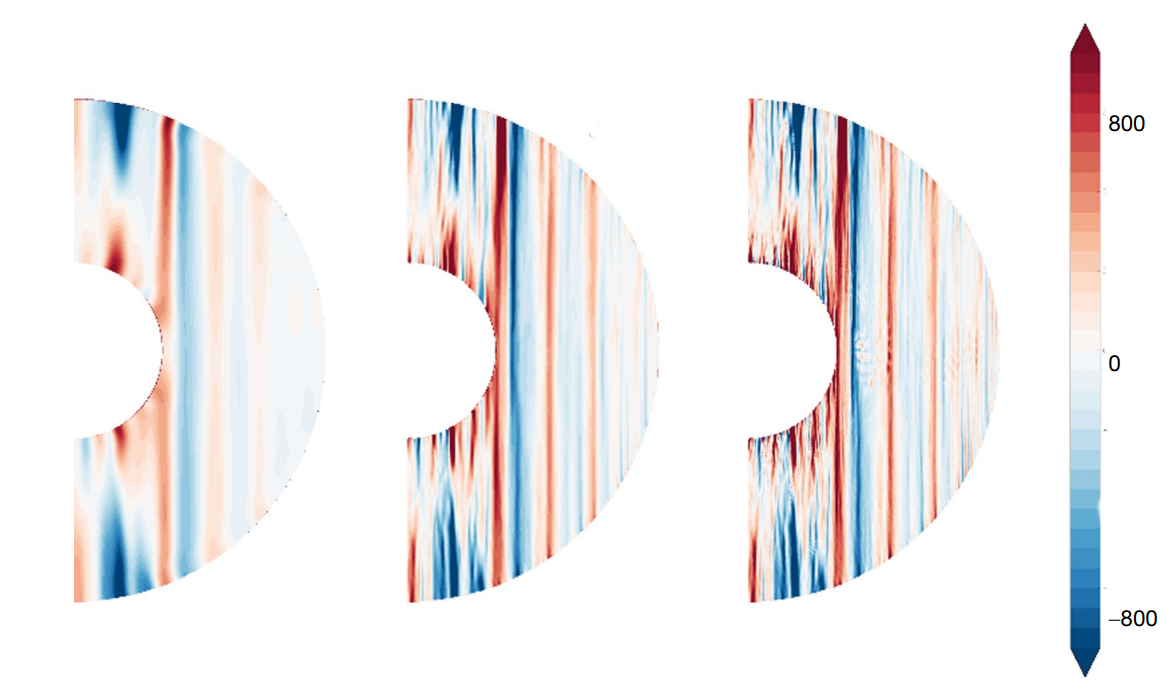
\includegraphics[width=\linewidth]{elements/qg_ground.png}
		\end{figure}
	\end{column}
	\end{columns}
\end{frame}

\begin{frame}{PG, QG, and all the geostrophic models}
\begin{columns}
	\begin{column}{.45\linewidth}
		How to exploit the \textcolor{ETHRed}{"near"-geostrophy}?
		\vspace{1em}

		We can choose an ansatz for the flow that is close to geostrophic flow.
		\vspace{1em}

		\textcolor{gray}{Also other options}
	\end{column}
	\begin{column}{.45\linewidth}
		Strictly geostrophic
		\[
			\mathbf{u} = \nabla\times (\Psi \hat{\mathbf{z}})
		\]
		does not satisfy non-penetrating BC.
		\vspace{.5em}
		\pause

		Geostrophic + vertical flow at boundary
		\[
			\mathbf{u} = \nabla\times (\Psi \hat{\mathbf{z}}) + \mathbf{u}_z
		\]
		does not satisfy divergence-free.
		\vspace{.5em}
		\pause

		\textcolor{ETHBlue}{Schaeffer and Cardin QG ansatz}
		\[
			\textcolor{ETHBlue}{\mathbf{u} = \frac{1}{H}\nabla\times (\Psi \hat{\mathbf{z}}) + \frac{z}{sH^2} \frac{dH}{ds} \frac{\partial \Psi}{\partial \phi} \hat{\mathbf{z}}}
		\]
		\textcolor{ETHBlue}{non-penetration + divergence-free.}
	\end{column}
\end{columns}
\end{frame}

\begin{frame}{PG, QG, and all the geostrophic models}
	Plesio-Geostrophy (PG) \parencite{jackson_plesio-geostrophy_2020} is built on the QG ansatz by Schaeffer and Cardin.

	In the absence of magnetic diffusion, PG converts
	\vspace{1em}

	\begin{columns}
	\begin{column}{.35\linewidth}
		Vector fields $\textcolor{ETHRed}{\mathbf{u}(\mathbf{r})}$ and $\textcolor{ETHRed}{\mathbf{B}(\mathbf{r})}$ living in \textcolor{ETHRed}{3D space}, 
		
		along with their evolution equations (Navier-Stokes + magnetic induction eqs)
	\end{column}
	\begin{column}{.18\linewidth}
		$\longrightarrow$ exactly to $\longrightarrow$
	\end{column}
	\begin{column}{.35\linewidth}
		15 PG quantities: \textcolor{ETHBlue}{$\Psi$, $\overline{B_s^2}$, $\overline{B_{\phi}^2}$, $\overline{B_sB_{\phi}}$, $\widetilde{B_sB_z}$, $\widetilde{B_\phi Bz}$, $\widetilde{zB_s^2}$, $\widetilde{zB_\phi^2}$, $\widetilde{zBsB_\phi}$, $B_{es}$, $B_{e\phi}$, $B_{ez}$, $B_{es,z}$, $B_{e\phi,z}$, $B_r$}

		all of which live in \textcolor{ETHBlue}{2D space},
		along with their evolution equations.
	\end{column}
	\end{columns}
\end{frame}

\begin{frame}{How did I end up here?}
    Since the start of my doctoral studies, I
    \begin{itemize}
        \item studied surface operators and tried to derive the boundary terms in the diffusive torsional oscillation (TO) equation for \textcolor{ETHBlue}{2 months} $\Longrightarrow$ didn't lead anywhere;
        \item studied torsional Alfvén waves and calculated the 1-D eigenmodes of the torsional oscillation for \textcolor{ETHBlue}{2 month} $\Longrightarrow$ didn't lead anywhere;
        \item studied anelastic approximation for \textcolor{ETHBlue}{1 month} in order to work on the anelastic version of QuICC, which may help the Jupiter simulation $\Longrightarrow$ project was called off and deemed unpromising before I could start to think about the numerics;
        \item picked up the thread and studied the reflection of Alfvén waves at the fluid-solid interface for \textcolor{ETHBlue}{2 months} $\Longrightarrow$ wrote a sixty-page document and yet had more questions than before;
        \item have been mainly working on the PG model since Aug 2023.
    \end{itemize}
\end{frame}

\section{The old implementation}
\begin{frame}{The old implementation - code \textit{Daria}}
    Mathematica implementation (previous member of the group, Dr. Daria Holdenried-Chernoff)
    \begin{figure}
        \centering
        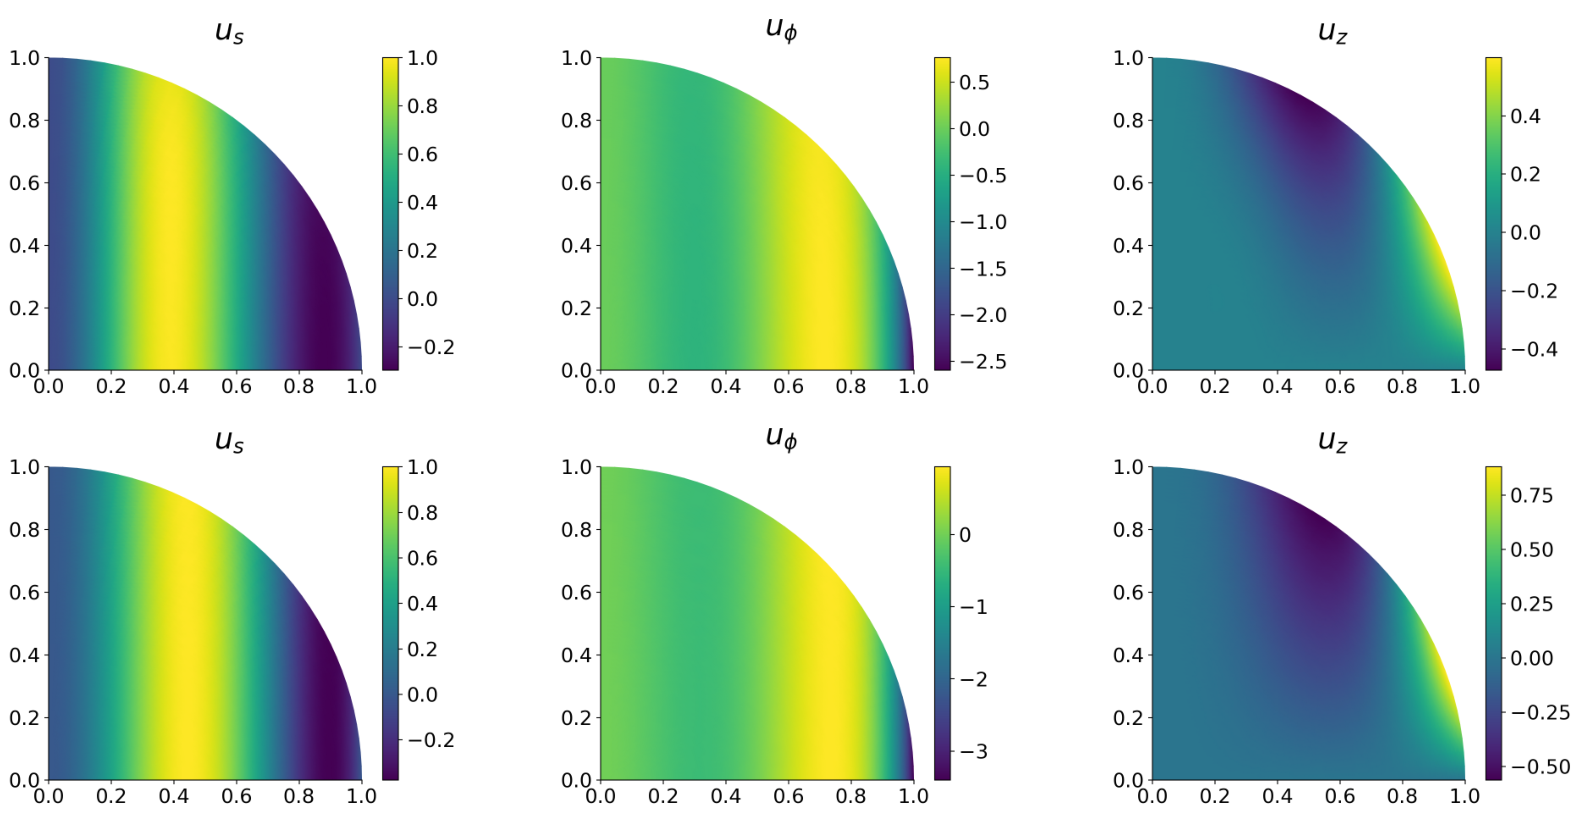
\includegraphics[width=.6\linewidth]{elements/Daria__toroidal_bg_eigen1033-922.png}
        \caption{Eigenmodes calculated using 3-D code \textit{Jiawen} (top) and PG code \textit{Daria}.}
    \end{figure}
    \textcolor{red}{Why reinvent the wheels when we already have a functioning implementation?}
\end{frame}

\begin{frame}{The old implementation - code \textit{Daria}}
    Citizens of Gotham, riddle me this... what is this code snippet doing?
    \begin{figure}
        \centering
        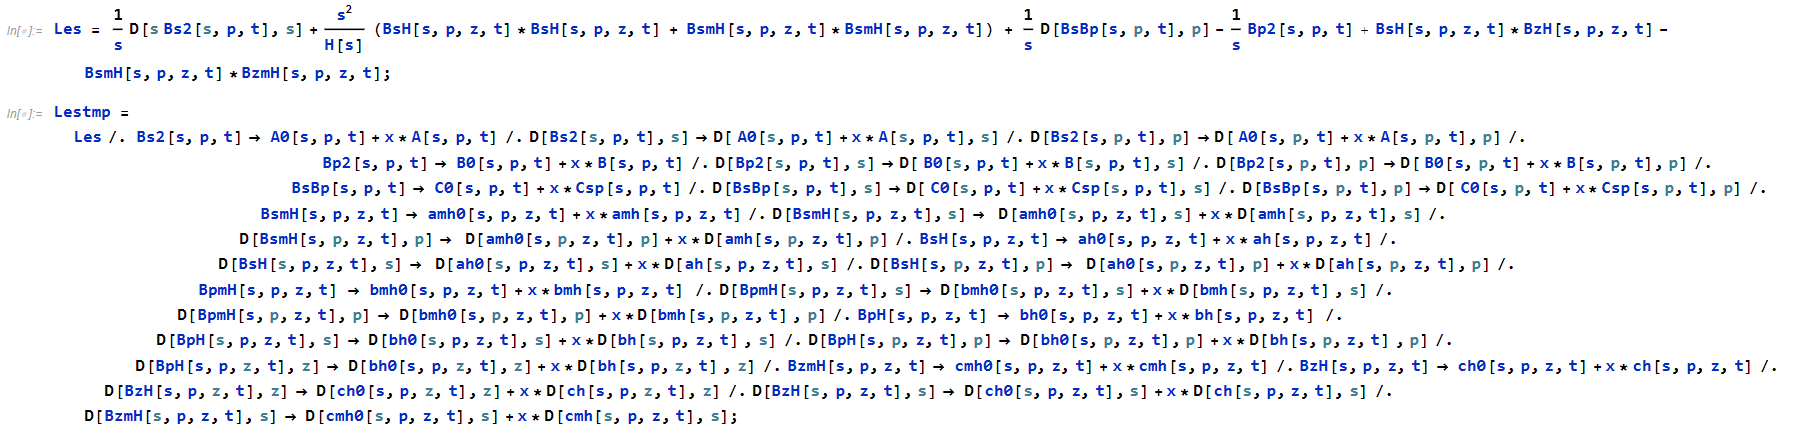
\includegraphics[width=\linewidth]{elements/Mathematica_snippet_1.png}
    \end{figure}
	\pause
	This rewrites the magnetic quantities in Lorentz force $\overline{L_\phi}$ as background + perturbation for linearization.

	e.g. \texttt{Bp2[s, p, t]->B0[s, p, t] + x*B[s, p, t]} equals to $\overline{B_\phi^2} = \overline{B_\phi^2}_0 + \epsilon \overline{B_\phi^2}'$
\end{frame}

\begin{frame}{The old implementation - code \textit{Daria}}
	\begin{columns}
	\begin{column}{.6\linewidth}
		\begin{figure}
			\centering
			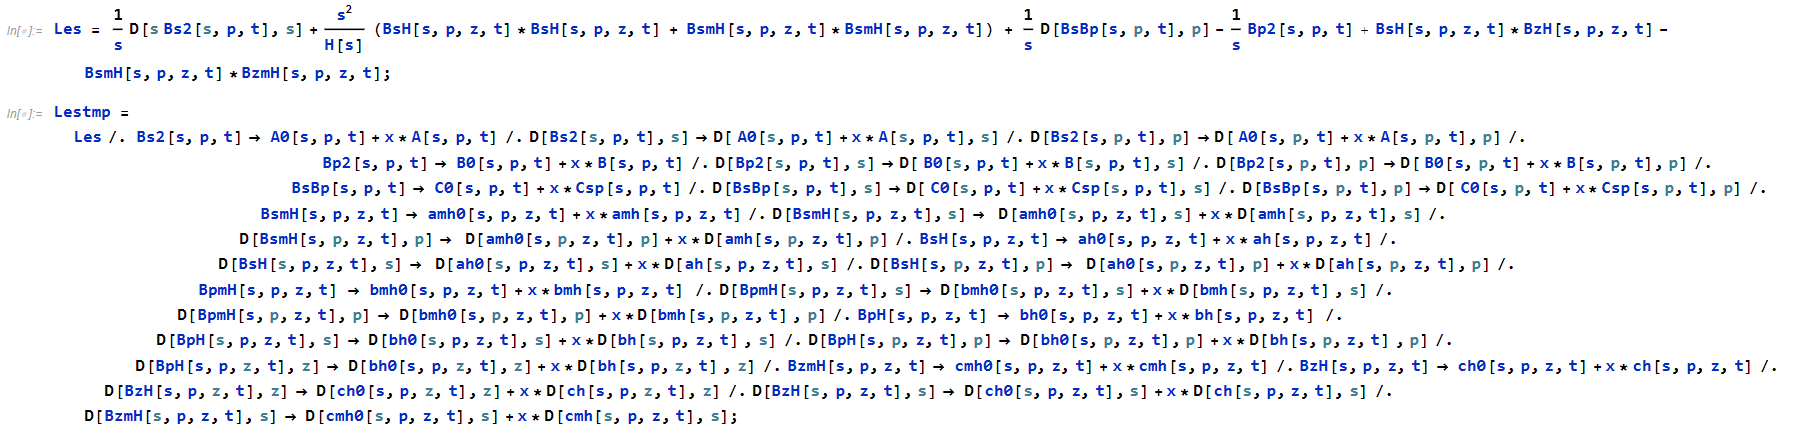
\includegraphics[width=\linewidth]{elements/Mathematica_snippet_1.png}
		\end{figure}
		Why is the code undesirable for \textcolor{ETHRed}{developers} and \textcolor{ETHBlue}{users} alike?
		\begin{itemize}
			\item long, repetitive operations $\Longrightarrow$ hard to \textcolor{ETHRed}{debug}
			\item namings: the background and perturbation fields are named from \texttt{A} to \texttt{H} $\Longrightarrow$ hard to \textcolor{ETHRed}{debug} or \textcolor{ETHBlue}{invoke}.
			\item At some point I even need a correspondence table to decipher the code.
		\end{itemize}
	\end{column}
	\pause
	\begin{column}{.4\linewidth}
		\begin{figure}
			\centering
			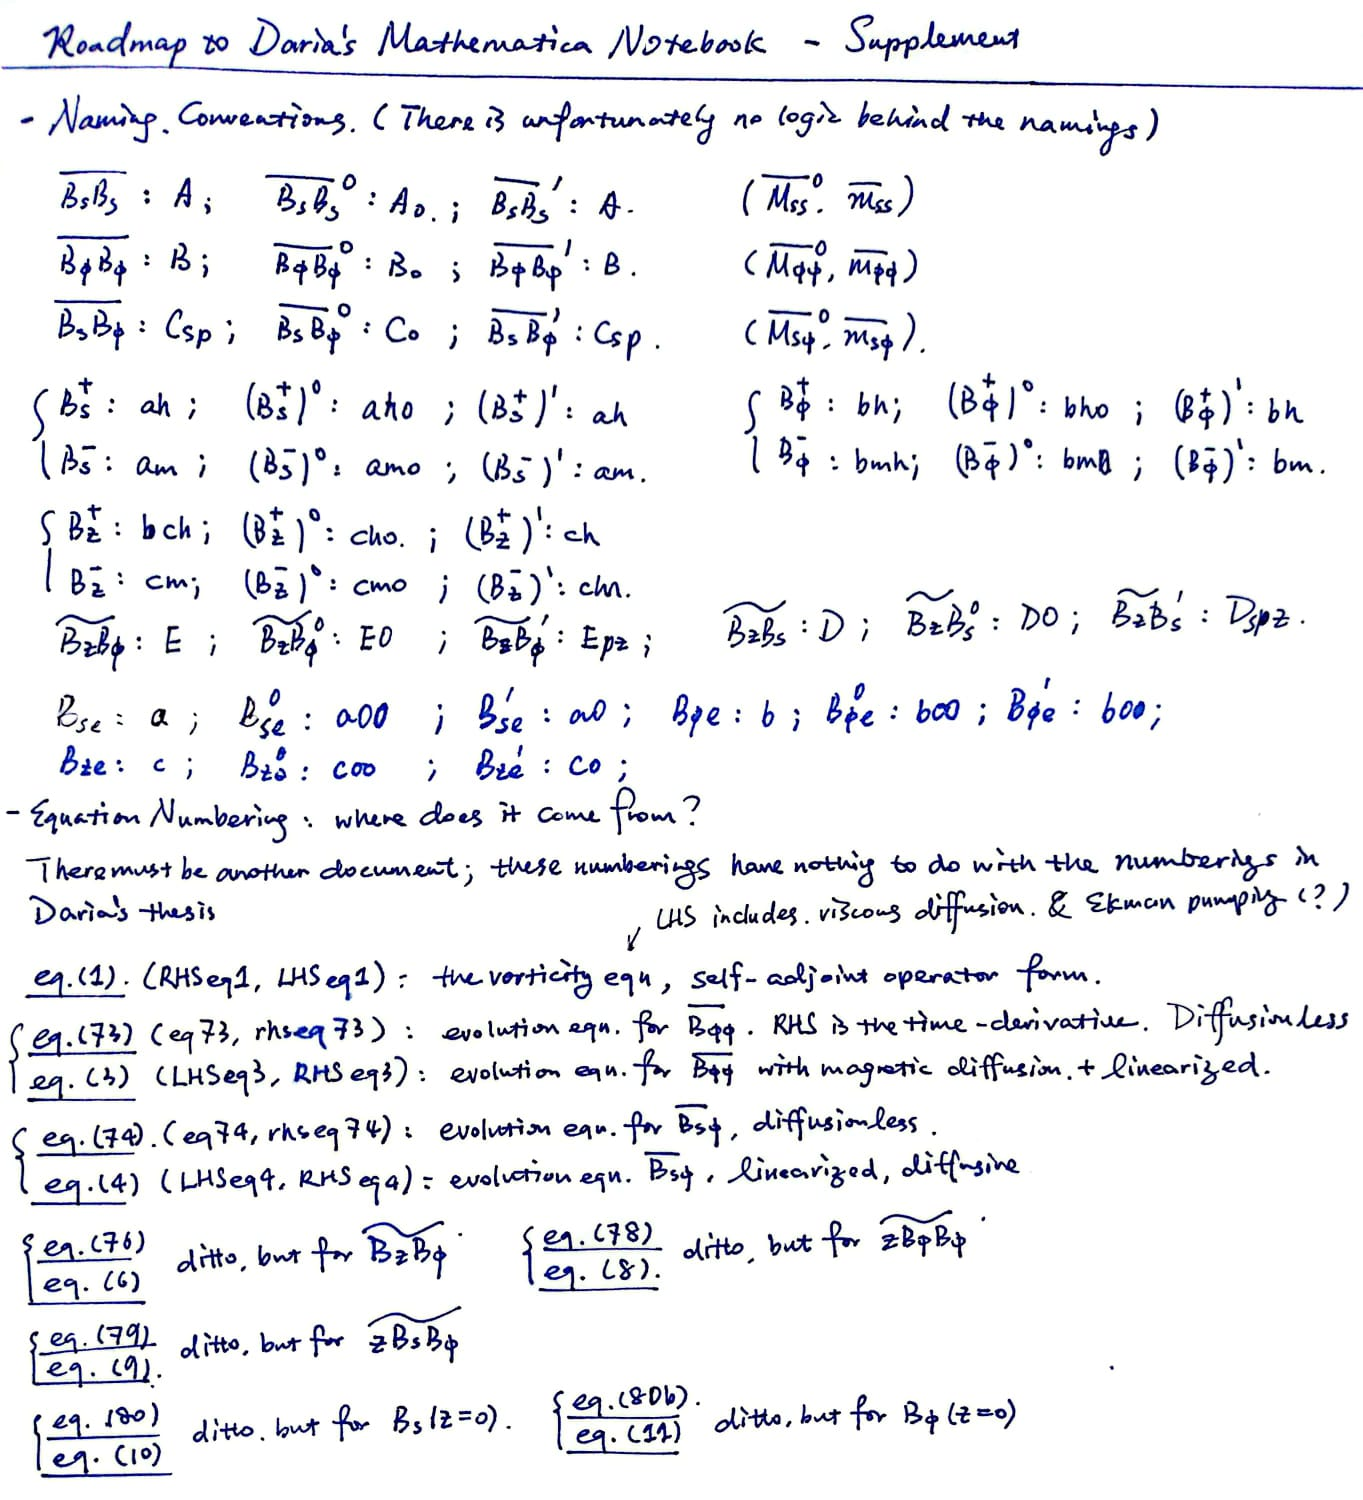
\includegraphics[width=.9\linewidth]{elements/correspondence_table.jpeg}
			\caption{List of physical variables and their names in the code.}
		\end{figure}
	\end{column}
	\end{columns}
\end{frame}

\begin{frame}{The old implementation - code \textit{Daria}}
\begin{columns}
\begin{column}{.46\linewidth}
    \begin{figure}
        \centering
        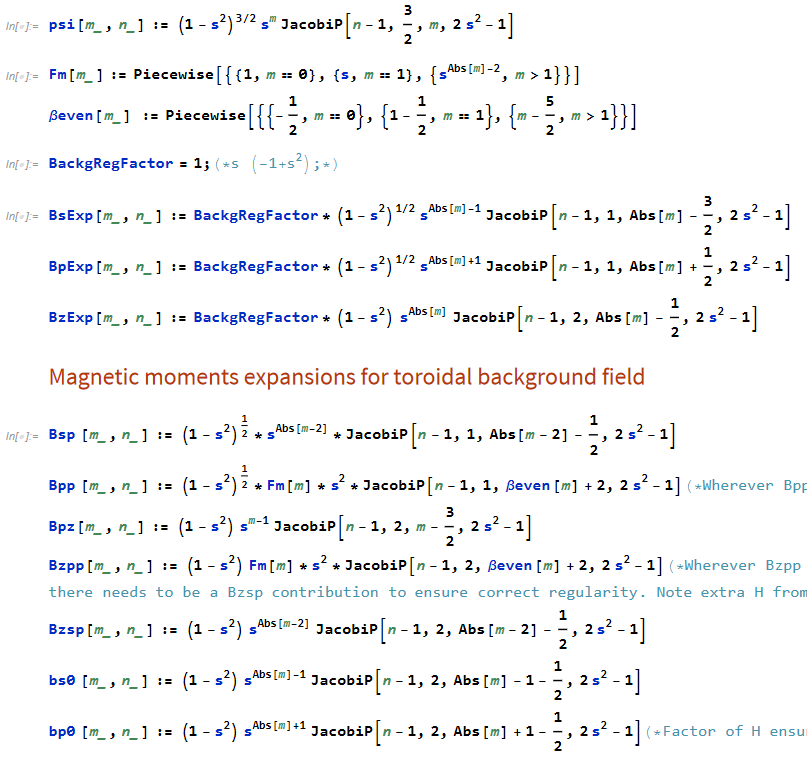
\includegraphics[width=\linewidth]{elements/Mathematica_snippet_expansion.png}
    \end{figure}
\end{column}
\begin{column}{.46\linewidth}
	Inflexible expansions: the expansion and the construction of matrices are hard coded in each notebook.
	\vspace{1em}

	To change the expansion, one needs to 
	\begin{itemize}
		\item produce a complete new Mathematica notebook;
		\item manually change the way the code collects the matrix elements.
	\end{itemize}
	\vspace{1em}

	Especially cumbersome to implement coupling, or if the bases do not coincide with the field quantities (more detail later).
\end{column}
\end{columns}
\end{frame}

\begin{frame}{The old implementation}
	\begin{columns}
	\begin{column}{.46\linewidth}
		Other problems
		\begin{itemize}
			\item The code is not efficient numerically, nor easily linked to efficient numerical libraries.
			\item Cryptic Mathematica syntax sugars
			\begin{figure}
				\centering
				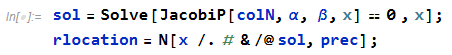
\includegraphics[width=.9\linewidth]{elements/Mathematica_snippet_3.png}
			\end{figure}
			\item When something unexpected happens, difficult to understand the cause
			\item Or perhaps I just don't like Mathematica
		\end{itemize}
	\end{column}
	\begin{column}{.46\linewidth}
		\begin{figure}
			\centering
			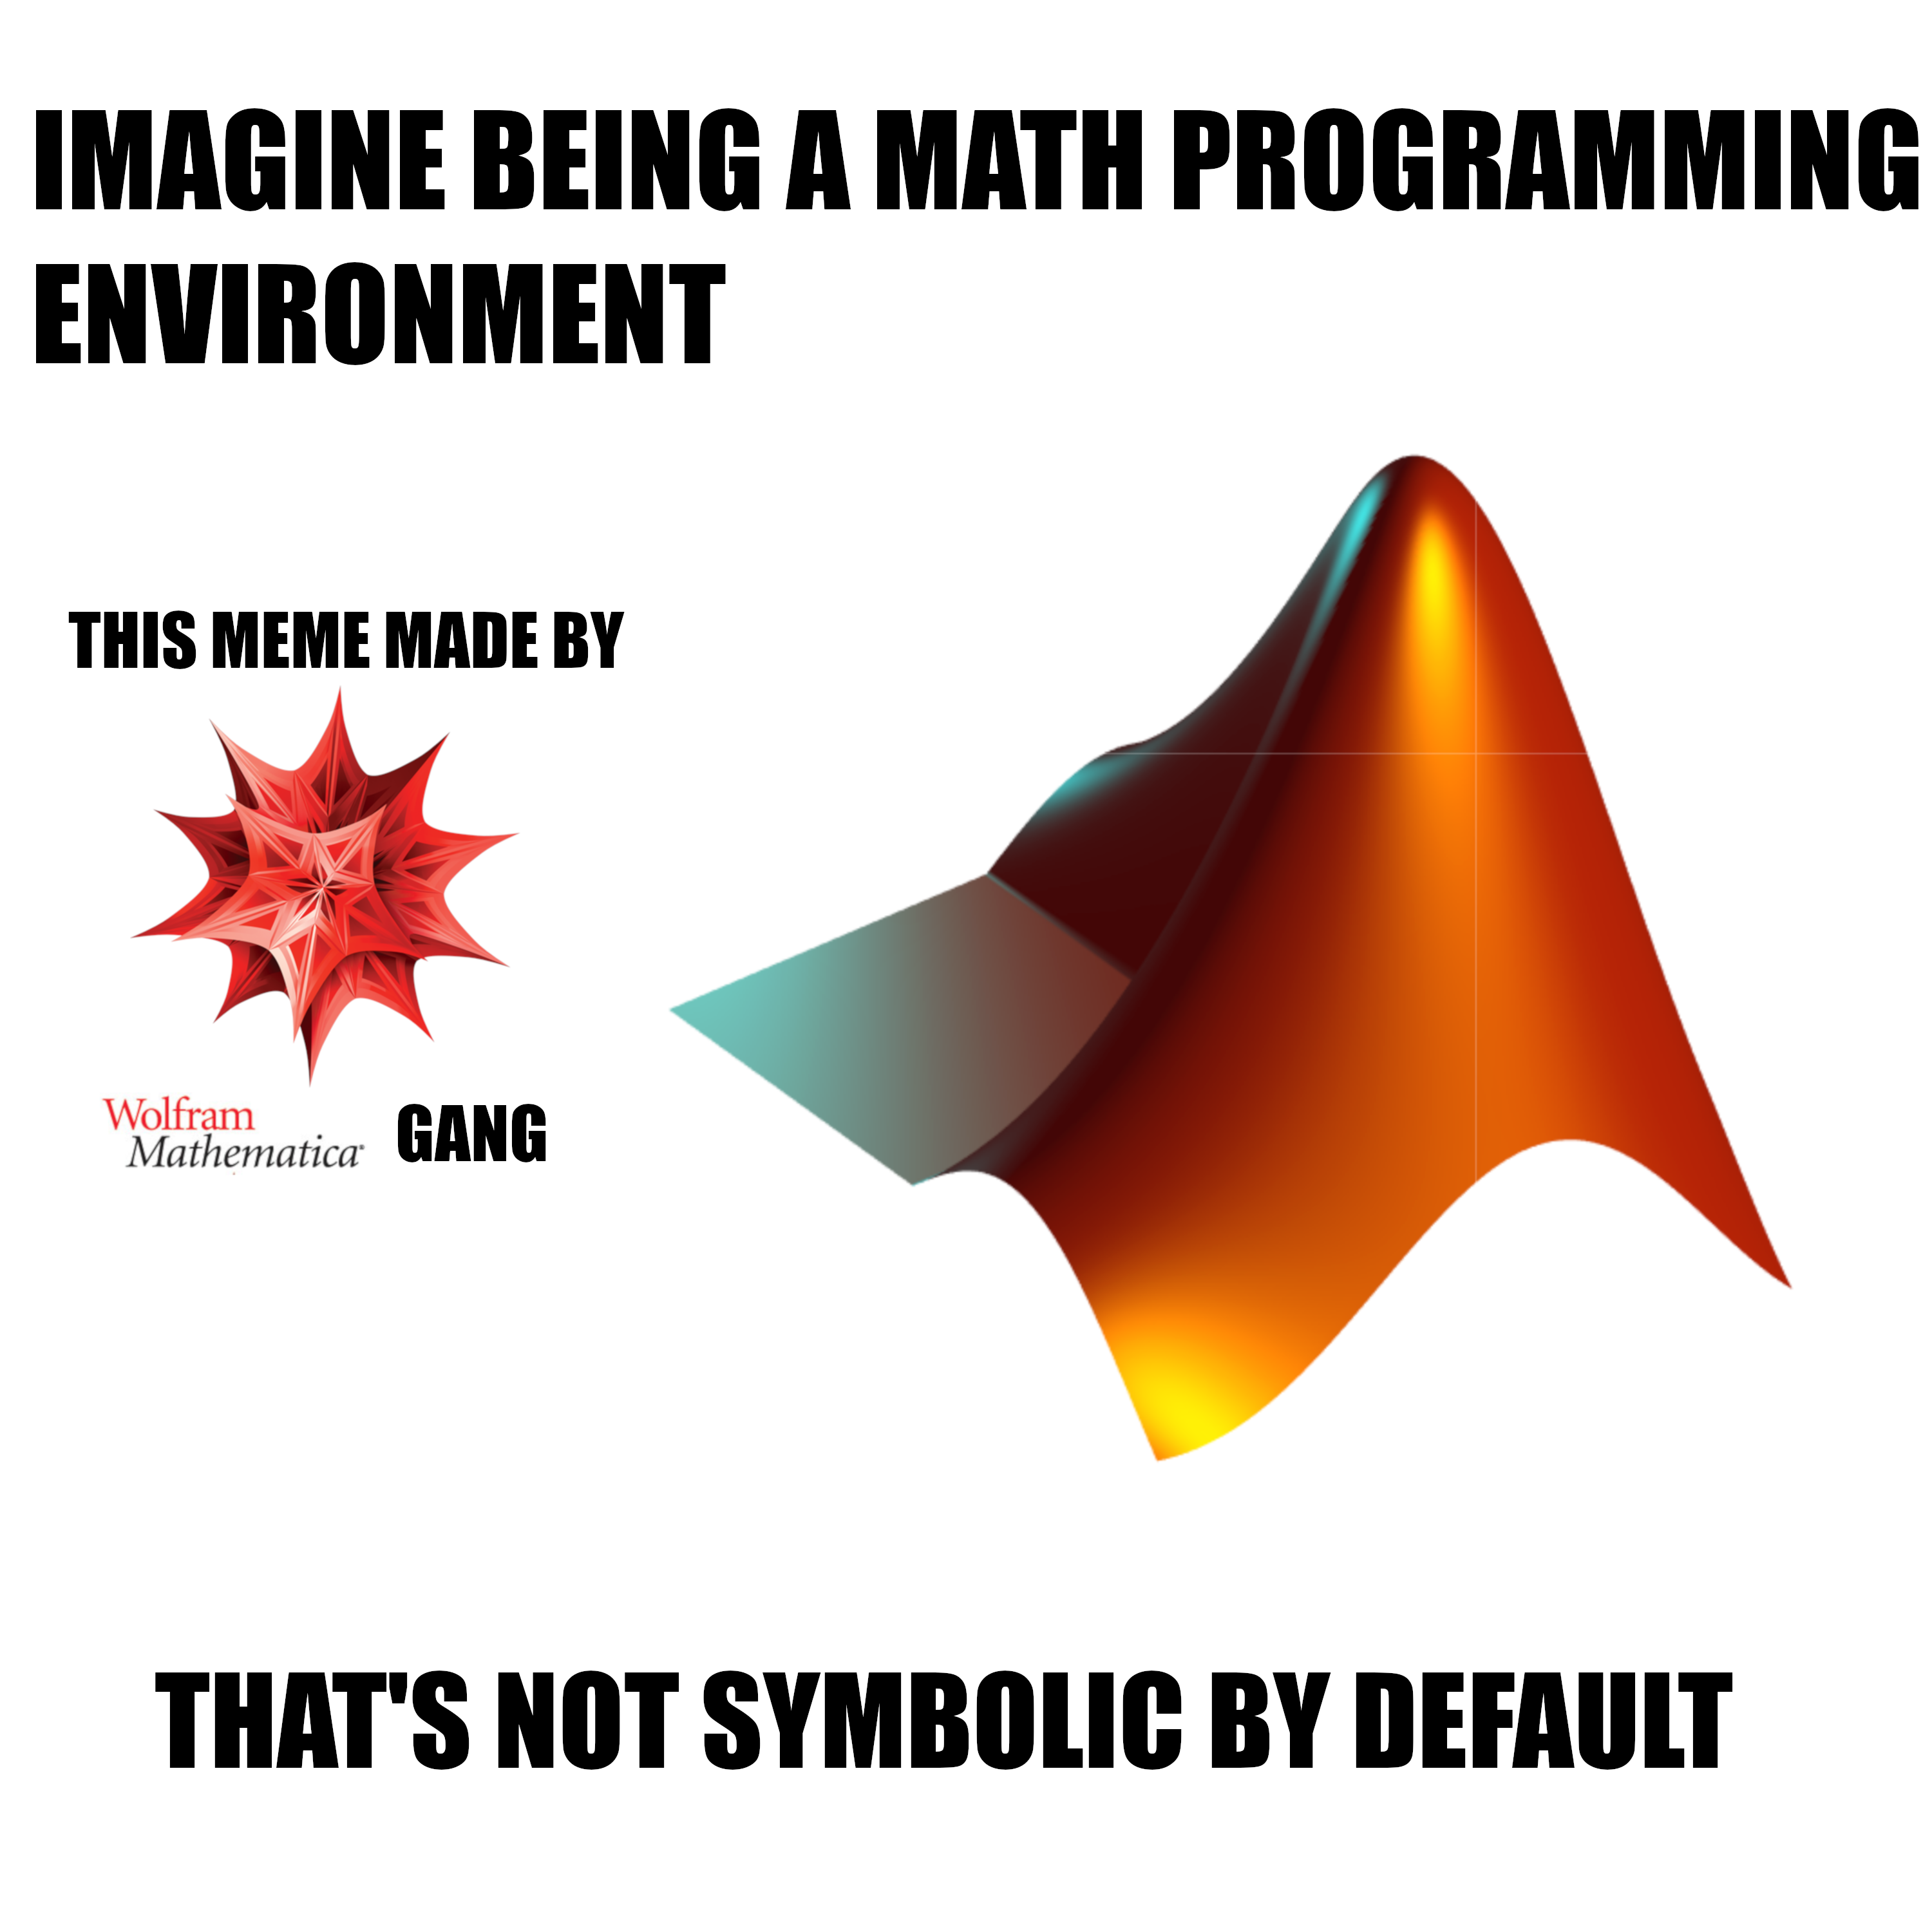
\includegraphics[width=\linewidth]{elements/mathematica_matlab_meme.png}
		\end{figure}
	\end{column}
	\end{columns}
\end{frame}

\section{Introducing PlesioGeostroPy}
\begin{frame}{Introducing PlesioGeostroPy}
    Make Plesio-Geostrophy model easy to use!
	\vspace{2em}

	\begin{columns}[t]
	\begin{column}{.32\linewidth}
		Symbolic manipulation

		[\texttt{sympy}]
		\begin{itemize}
			\item all PG equations stored, easily accessible
			\item linearization
			\item configure expansion
			\item collect matrix elements
		\end{itemize}
		\vspace{1em}

		Demo notebook available.
	\end{column}
	\begin{column}{.32\linewidth}
		Numerical computation

		[\texttt{mpmath},\texttt{numpy}/\texttt{scipy}]
		\begin{itemize}
			\item compute matrix elements
			\item quadrature
			\item eigenvalue solver
			\item \textcolor{gray}{time stepper}
			\item comes in both std (\texttt{numpy}+\texttt{scipy} backend) and multi-precision (\texttt{mpmath})
		\end{itemize}
	\end{column}
	\begin{column}{.25\linewidth}
		Post-processing

		[\texttt{matplotlib}]
	\end{column}
	\end{columns}
\end{frame}

\begin{frame}{First batch of result: a glimpse of efficiency}
	\begin{columns}
	\begin{column}{.4\linewidth}
		Test problem: eigenvalue problem with Malkus background field, diffusionless.
		\vspace{1em}
		
		A not-so-well-controlled test:

		Assemble mass and stiffness matrices at the size of $124\times 124$ (PlesioGeostroPy) and $73\times 73$ (Mathematica)
		\vspace{1em}

		Three versions:
		\begin{itemize}
			\item Code Daria, eval to 32nd digit
			\item PlesioGeostroPy, multiprecision eval (same precision)
			\item PlesioGeostroPy, scipy eval (double precision)
		\end{itemize}
	\end{column}
	\begin{column}{.55\linewidth}
		\begin{table}
			\caption{Time lapse for computing mass and stiffness matrices}
			\begin{tabular}{lll}
				\toprule
				Code (version) & Time $\mathbf{M}$ & Time $\mathbf{K}$ \\ 
				\midrule
				Code Daria Mathematica & 5s & 50s* \\ 
				PlesioGeostroPy-mp32 & 16s & 35s \\ 
				PlesioGeostroPy-scipy & 400ms & 750ms \\
				\bottomrule
			\end{tabular}
		\end{table}
		*{\scriptsize may not be representative as this involves other operations}

	\end{column}
	\end{columns}
\end{frame}

\begin{frame}{First batch of result: eigenvalues with Malkus background field}
	\begin{columns}
	\begin{column}{.32\linewidth}
		Test: eigenvalue problem with Malkus background field, diffusionless.
		\vspace{1em}

		Eigenvalues (right) are computed for $\mathrm{Le}=10^{-4}$, the errors are measured relative to the analytical eigenvalue for the PG model.
		\vspace{1em}

		\texttt{PlesioGeostroPy} $\sim$ Code \textit{Daria}
		
		mp32 $\approx$ scipy.
	\end{column}
	\begin{column}{.6\linewidth}
		\begin{figure}
			\centering
			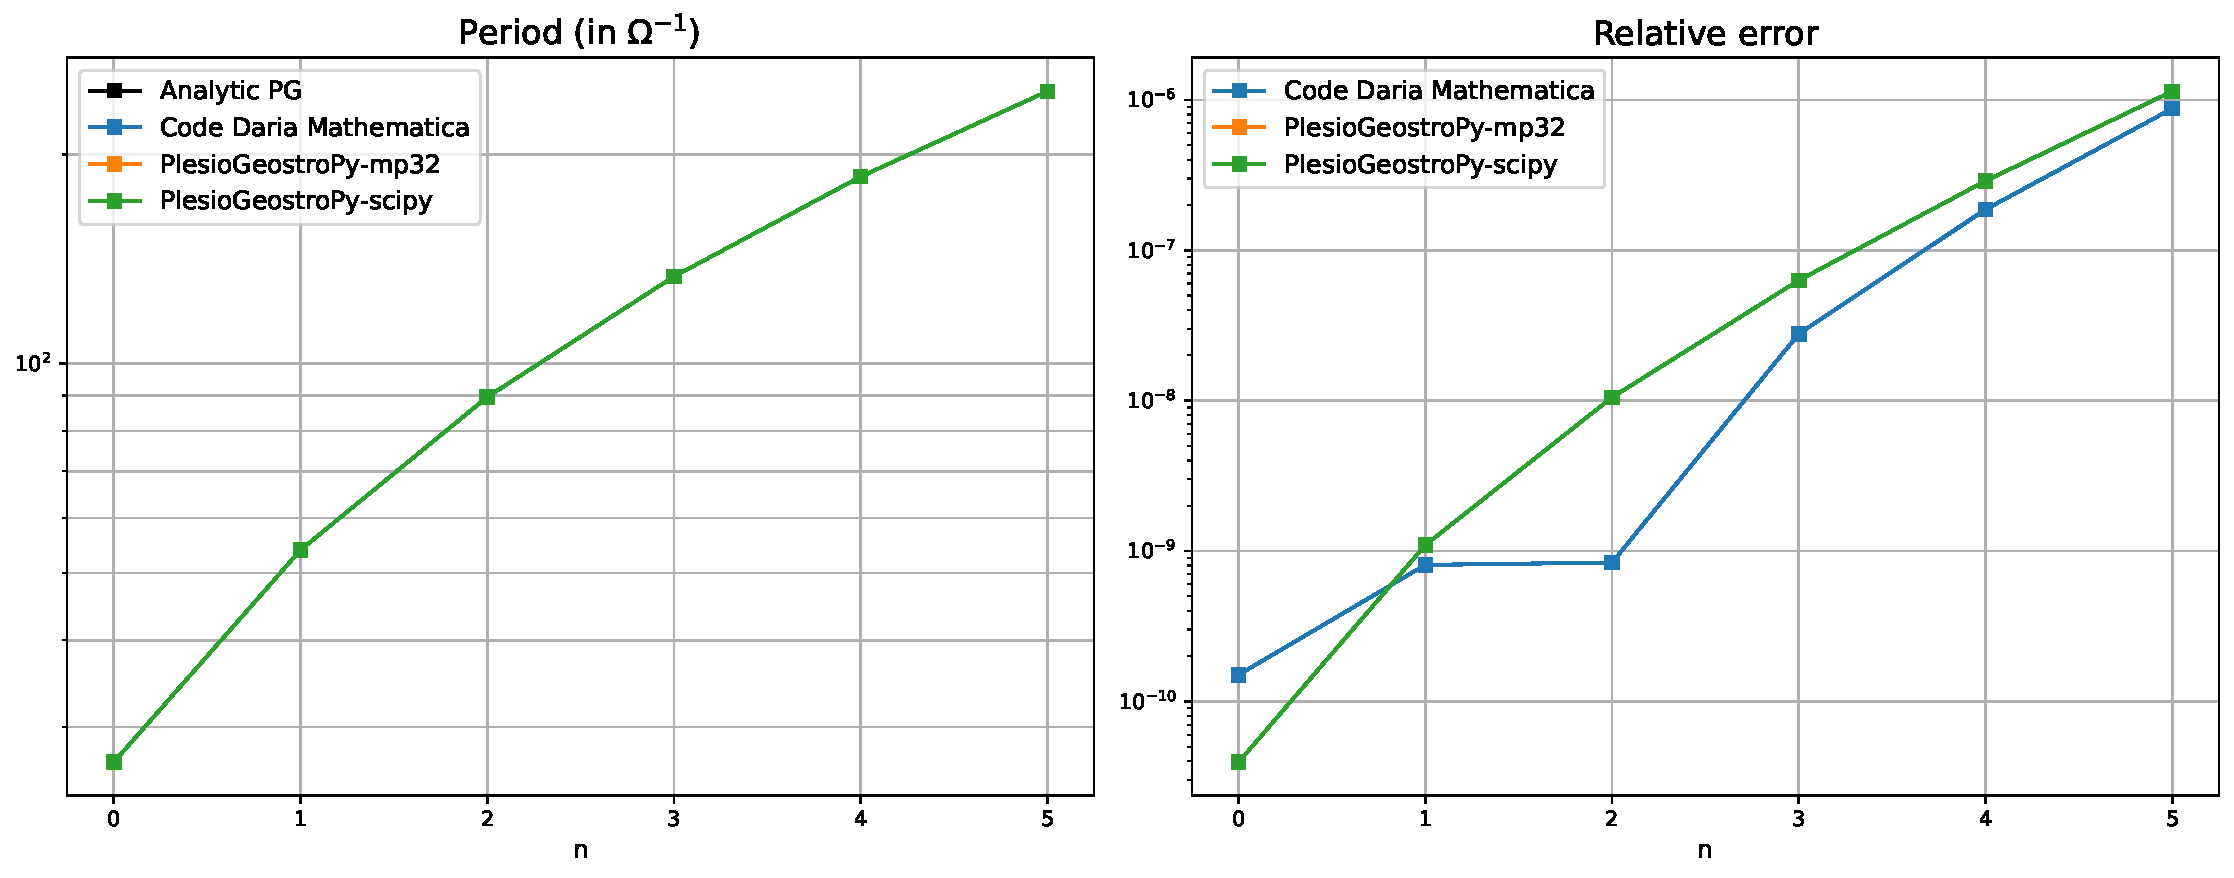
\includegraphics[width=.9\linewidth]{../out/imgs/err_comparison_east__PG.pdf}
			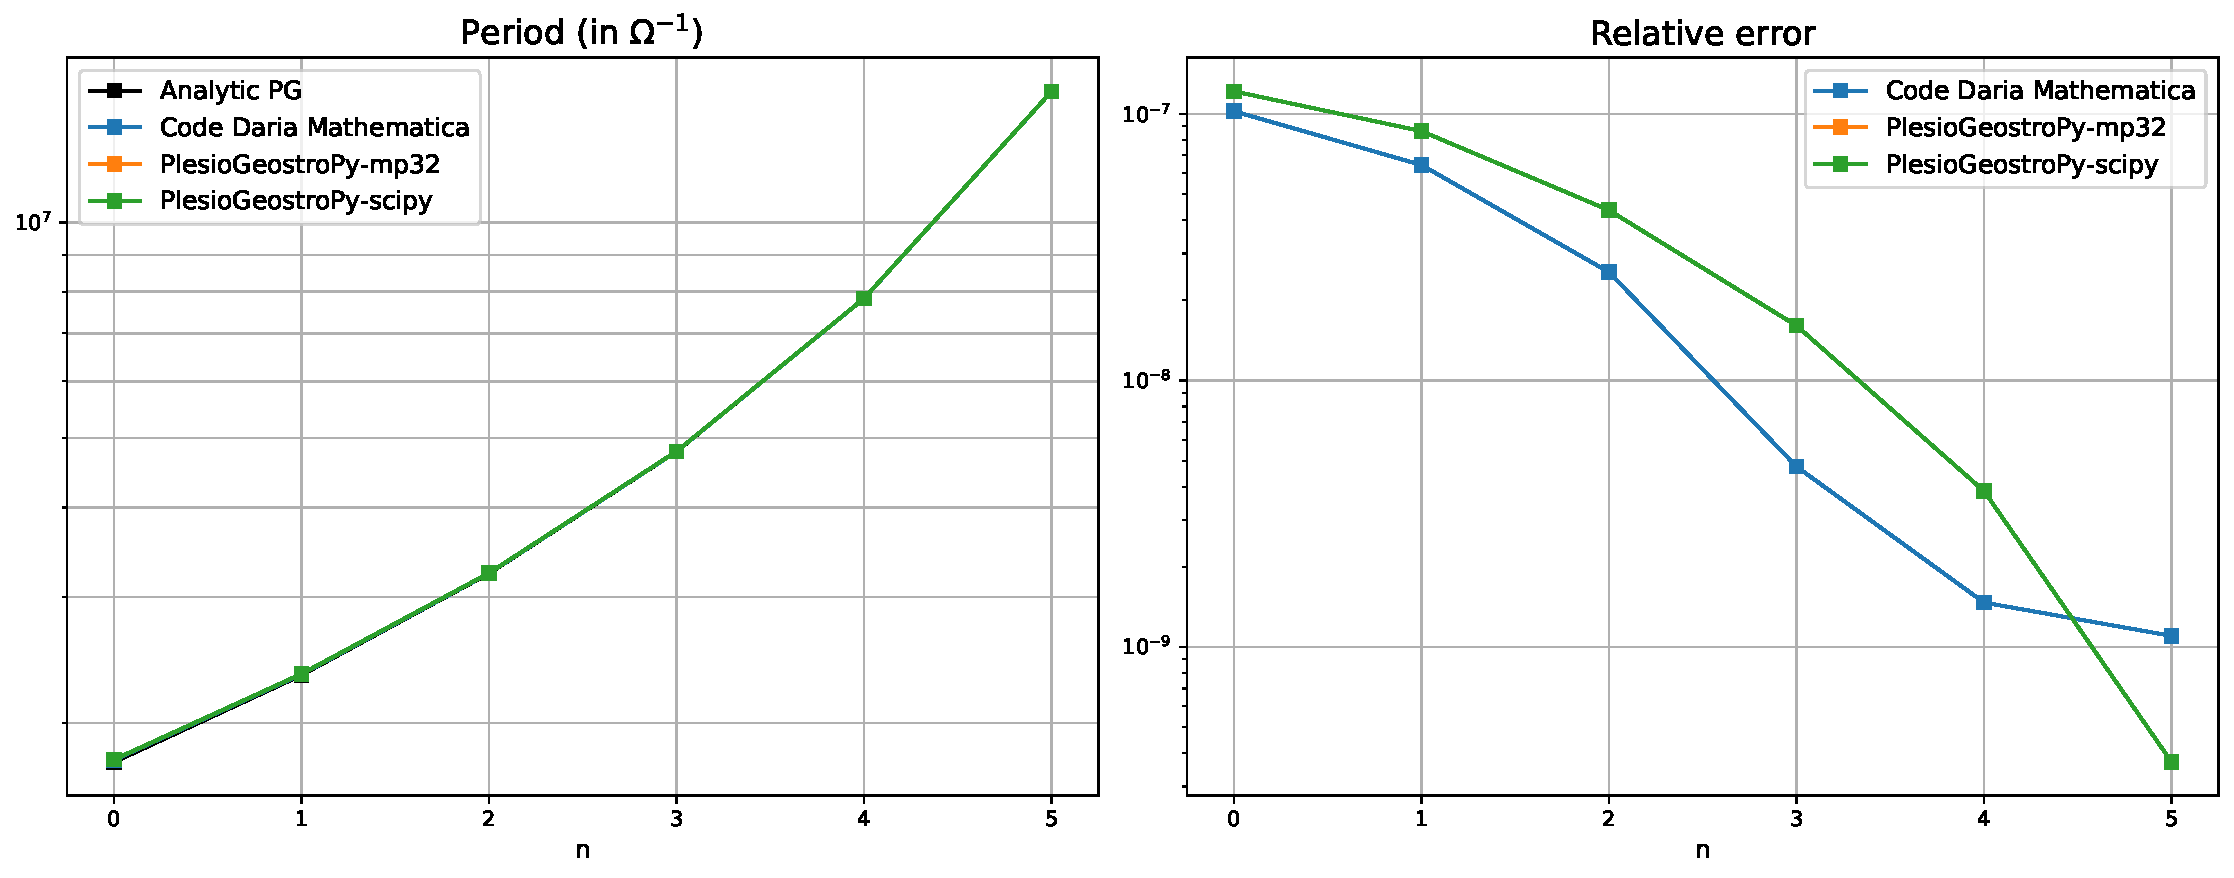
\includegraphics[width=.9\linewidth]{../out/imgs/err_comparison_west__PG.pdf}
			\caption{Periods and errors of the lowest 6 eigenmodes for the fast(top) and slow(bottom) branch.}
		\end{figure}
	\end{column}
	\end{columns}
\end{frame}

\begin{frame}{First batch of result: eigenmodes with Malkus background field}
	\begin{columns}
		\begin{column}{.32\linewidth}
			Test: eigenvalue problem with Malkus background field, diffusionless.
			\vspace{1em}
	
			Eigenmodes are computed for $\mathrm{Le}=10^{-4}$.

			Right fig. shows the equatorial sections of the 5-th eigenmode for $m=3$.
		\end{column}
		\begin{column}{.6\linewidth}
			\begin{figure}
				\centering
				\includegraphics[width=.9\linewidth]{../out/solutions/Malkus/m3n5_sympy_eqplot.png}
			\end{figure}
		\end{column}
	\end{columns}
\end{frame}

\begin{frame}{First batch of result: eigenmodes with Malkus background field}
	\begin{columns}
		\begin{column}{.32\linewidth}
			Test: eigenvalue problem with Malkus background field, diffusionless.
			\vspace{1em}
	
			Eigenmodes are computed for $\mathrm{Le}=10^{-4}$.
		\end{column}
		\begin{column}{.6\linewidth}
			\begin{figure}
				\centering
				\includegraphics[width=\linewidth]{../out/solutions/Malkus/m3n5_sympy_mdplot.png}
				\caption{Meridional sections of the velocity field components for the 5-th eigenmode for $m=3$.}
			\end{figure}
		\end{column}
	\end{columns}
\end{frame}

\section{Future works}

\begin{frame}{To-do list}
	\begin{itemize}
		\item Alternative expansions (even alternative evolution equations)
		\begin{itemize}
			\item Additional coupling revealed (before group retreat), unlikely to implement all low-order coupling in the current way.
			\item Need some thoughts + pen-and-paper derivation.
		\end{itemize}
		\item Reduced systems of the eigenvalue problems
		\begin{itemize}
			\item The eigenvalue problem with $\mathbf{u}^0 = 0$ can always be reduced to a problem with two variables, instead of 15.
		\end{itemize}
		\item Treatment of the $B_r$
		\begin{itemize}
			\item Circumvented in the eigenvalue problem.
			\item Required for time stepping.
			\item Possible to incorporate other than insulating BC?
		\end{itemize}
		\item Time step the system
	\end{itemize}
\end{frame}


\end{document}